\setlength{\headheight}{14.49998pt}
\chapter{}\label{ch:functionalities}

This chapter consists of a detailed view over the concept and functional requirements of the CASCIFFO platform.
It is structured with the following sections:
\begin{itemize}
    \item Related work: Analysis of platforms with similar functionalities.
    \item Infrastructure: Description of technologies and framework used for the development of CASCIFFO. 
    \item Access control: Identification and categorization of actors and their roles.
    \item Processes: Identification and detailing of the process flow.
    \item Functional Requirements: Description of functional requirements.
\end{itemize}

\section{Related work}
Clinical trial management is an important factor to consider for any health care organization, to be able to track and manage any data concerning clinical trials and studies, from the moment of the proposal, to the clinical trial itself, the patient recruitment and monitoring management. To this effect, after an brief search and analysis of platforms providing these features, two platforms stood out: the Clinical Conductor Clinical Trial Management System (CTMS)~\cite{clinical-conductor-ctms} by Advarra~\cite{Advarra} and RealTime-CTMS. Clinical Conductor CTMS is a premium service scalable to optimize finances, regulatory compliance, and overall clinical research operations such as financial, patient and visit management including patient recruitment. The platform RealTime-CTMS is a leader in cloud-based software solutions for the clinical research industry and is dedicated to solving problems and providing systems that make the research process more efficient and more profitable~\cite{realtime-ctms}.
CASCIFFO takes a tailored approach in building a straightforward platform that fits the needs of the Hospital Professor Doutor Fernando Fonseca. It features, in similarity to the aforementioned platforms, clinical trial management, from the moment its a proposal to the end of the clinical trial, allowing the entire progress to be tracked and analyzed; time line management in the aspect of tracking progress and reporting the completion date as well as possible overdue target dates; patient monitoring and visit management; financial management of clinical trials and each individual member of the investigation team and a role-based system for users of different internal departments. Furthermore the way CASCIFFO is planned to be developed, will allow for offline use. It is not as robust as a leading cloud-based software solution like RealTime-CTMS, however, it accomplishes its purpose of bringing innovation and simplicity to the management of clinical trials of the Hospital Professor Doutor Fernando Fonseca's Clinical Research Unit (Unidade de Investigação Clínica).

\section{Infrastructure}
\label{sec:infrastructure}
The infrastructure of CASCIFFO, as mentioned previously, consists of two core modules, the front-end and the back-end.  
The front-end runs on a Node.js environment, using \href{https://reactjs.org/}{React}, a Javascript library for building user interfaces~\cite{reactjs},  with Typescript to build all front-end functionalities. The dependencies are managed and installed using \href{https://docs.npmjs.com/about-npm}{npm}, a software package manager, installer and the worlds largest software library~\cite{npm}. npm was chosen over \href{https://yarnpkg.com/}{yarn}~\cite{yarn} due to its larger community and support.
The back-end executes on a run-time Java environment, utilizing Spring-boot and Spring-webflux as the basis for building the server. Spring-boot facilitates the building and deployment of web applications by removing much of the boilerplate code and configuration associated with web development~\cite{spring-boot}. Spring-webflux, despite being a new technology, was chosen for its non-blocking webstack framework~\cite{spring-webflux}. This technology allows for the use of Spring Data R2DBC~\cite{r2dbc}, a driver that overcomes the inherent blocking limitation of drivers such as JDBC when accessing data in a database. The database connections via R2DBC are non-blocking, returning streams of data in the form of Flux and Mono upon access.
CASCIFFO has its own database, utilizing the framework \href{https://www.postgresql.org/about/}{PostgreSQL}, a powerful open-source object-relation database system. Postgres was chosen for its earned reputation in its proven architecture, reliability, data integrity and community support~\cite{postgresql}. While CASCIFFO has its own databse, the patient and medical staff data will be imported from an internal database, "Admission", within the HFF/UIC. There are restrictions on the amount of queries made on the medical staff information, limiting this procedure to once per day.

\section{Access control}
\label{sec:access-control}
Within the app CASCIFFO, in order for the management of clinical investigations to progress, it needs to be reviewed by many entities, such as the Administrative Council ("Concelho administrativo", CA), the Finance and Juridical department.
Given this nature of CASCIFFO, there needs to be a well-defined structure of access control, so that each entity can contribute to the management of clinical investigations within the scope of their responsibilities. Each involved entity must have a role and a set of permissions.  
The roles identified are as follows: the UIC role, given to the investigators who can create and edit clinical investigation proposals; the Team Member role, given to investigators belonging to the team conducting the clinical investigation; the Management role, able to approve and reject clinical investigation proposals; the Finance and Juridical roles, given to collaborators who's function belongs within the Finance and Juridical departments, respectfully; and finally the Superuser role, who has complete access to every feature CASCIFFO has to offer. Each user of CASCIFFO can only have one role.

\section{Processes} 
\label{sec:processes}
This section details the types of processes occurring within the scope of the project.  
There are three identified processes consisting of the life-cycle of a clinical investigation proposal, the Clinical Trials and the contract addenda. 



\subsection{Clinical Investigation Proposals}
\label{subsec:clinical-investigation-proposals}
From the instant a clinical investigation is kicked-off, it follows through a series of states and protocols that must be adhered to, in order to be completely validated.
There are two types of clinical investigations: Clinical Trials and Observational Trials.  
Each state, except the terminal one, has an entity responsible, `owner`, for advancing the state. 
The flow of states is as follows:  

\begin{enumerate}
    \item Submitted ("Submetido"), `owner=UIC`;
    \item Negotiation of financial contract ("Negociação de CF"), `owner=UIC`;
    \item Internal validation ("Validação interna"), `owner=Finance, Juridical`;
    \item External validation ("Validação externa"), `owner=UIC`;
    \item Submission to the CA ("Submissão ao CA"), `owner=UIC`;
    \item Internal validation ("Validação interna"), `owner=CA`;
    \item Validated ("Validado").
\end{enumerate}

The enumerated set of states corresponds to the life-cycle of a clinical trial Proposal. An Observational Trial Proposal consists of the enumerated states 1, 5, 6 and 7; it lacks a financial component and a promoter.  

Taking the example of the submission of a clinical trial Proposal, an investigator starts by creating and submitting a proposal. Once it's submitted, the CA will be notified, via app and email. This state is described as \textit{Submitted}.  
When the negotiation of the financial contract begins, the principal Investigator, who belongs to the UIC role, will advance the state to its next step in the proposal's evolution, \textit{Negotiation of financial contract}.
When the financial negotiation reaches an agreement of the UIC and external promoter, the investigator advances the state to its next stage, \textit{Internal validation}. Upon advancing, the users with the role of `Finance` and `Juridical`, which represents the Financial and Juridical internal departments, respectfully, will be notified that a proposal is ready to be evaluated. The evaluation will consist of a simple `Accept` or `Refuse` with added justification for the choice. In the case of either user with `Finance` or `Juridical` role reject the financial contract, the proposal's will backtrack to \textit{Negotiation of financial contract}, notifying the UIC of the occurrence.  
Once it's accepted by both roles, the proposal will automatically advance into the next state, \textit{External validation}. In this state the UIC will be notified of the change and asked to verify all the documents, including the final version of the financial contract. The UIC to the external promoter, requesting their signatures. When the reply is received via email, the UIC adds the received signatures and possible additional documents to the proposal in the CASCIFFO platform, advancing it to the next stage \textit{Submission to CA}.  
In the state \textit{Submission to CA}, the principal investigator will be notified both via the platform and email that a proposal requires their signature. Once the principal investigator submits their signature into the platform, he can advance the proposal's state into \textit{Internal Validation}. The progression to the mentioned state will notify users with the `CA` role stating that a proposal is ready for its final evaluation.  
Once a user with the role of `CA` checks the proposal he can either validate it or not. In case it's not validated, the proposal will become `canceled` with its life-cycle ending there, however, if it is validated, the proposal can become fully validated once the termination of another process is ends successfully.  
This process, which can be considered a sub-process, is called the validation protocol. It starts in parallel when the proposal is first submitted.  
The purpose of this protocol is to validate the clinical investigation's ethical and safety values. It consists in the validation of the proposal by internal and external agencies, the \href{https://www.ceic.pt/}{clinical investigations Ethics Comity ("Comissão de Ética para Investigação Clínica", CEIC~\cite{ceic})} and \href{https://www.infarmed.pt/web/infarmed}{INFARMED, I.P}~\cite{infarmed} respectfully. The protocol ends when either of the mentioned agencies approves or rejects the proposal.  
Once it has successfully passed through the described validation protocol, the proposal becomes \textit{Validated} and a Clinical or Observational Trial is automatically created, importing the core information from the proposal.  
If either process declares the proposal invalid, its state becomes `canceled`, notifying the UIC and showing the root cause of cancellation.

Each proposal is distinguished by six main properties, the principal investigator, the type of investigation, the type of therapeutic service it's integrated into (\textit{i.e.} Oncology), the `Sigla` which represents the name of the therapeutic or medicine, the partnerships involved in the investigation and the medical team participating in the investigation.  
Proposals with a financial component must also include the promoter of the investigation, in addition to the properties listed.  

\subsection{Clinical Trials} 
\label{subsec:clinical-trials}
The life-cycle of a clinical trial is divided into three states: active, completed, and canceled.  
Starting with the active state, a clinical trial will become available for viewing and editing once its proposal has been accepted. 
Clinical trials, as a process, consist on the experimentation of new medicine or treatment on a set of participants. These participants can be added to the clinical trial directly from the application. The experimentation requires constant monitoring, through visits, on each participant. These visits can be scheduled either when a participant is added or created afterwards.  
In addition to monitoring participants, several studies can be made in the scope of the clinical trial, such as scientific articles, presentations, reports, etc. 

\subsection{Addenda to the contract}
\label{subsec:addenda-process}
Throughout the life of a clinical trial, there can be made changes to the study's contract, be it changing the investigator team or other factors that impact the standard run of the study. These changes pass through two entities before being applied; the UIC and the CA.  
The addenda can only be made once a clinical trial is active, which means its proposal has already been approved.  
The addenda have five different states: submitted `Submetido`, internal validation by UIC `Validação interna`, internal validation by CA `Validação interna`, the terminal state validated `Validado` and finally the terminal canceled state `Indeferido`.  
The first four mentioned states are sequential, with the last one being an exception state. The sequential flow of states have an entity responsible for advancing their state, the `owner`. Listed below, in similar fashion to the states presented in the proposal process, is the aforementioned sequence:
\begin{enumerate}
    \item Submitted ("Submetido"), `owner=UIC`;
    \item Internal validation ("Validação interna"), `owner=UIC`;
    \item Internal validation ("Validação interna"), `owner=CA`;
    \item Validated ("Validado").
\end{enumerate}


\section{Functional Requirements}
\label{sec:functional-reqs}
This section details the functional requirements and presents a mock user interface (UI) that will satisfy the requirement.
The main features of CASCIFFO can be separated into three groups, which are: general functionalities, clinical component and financial component.  
\begin{enumerate}
    \item General features
        \begin{itemize}
            \item Visualization and management of Clinical Trials as a process; 
            \item Ability to edit and validate data (edit checks);
            \item Access control based on different user profiles; 
            \item Access by computer, tablet or smartphone; 
            \item Ability to export information in numerical or graphical mode; 
            \item Ability to customize the form of visualization.
        \end{itemize}
    \item Clinical Component
        \begin{itemize}
           \item View detailed characteristics and evolution of clinical trials including the tested medicine or technique in question;
           \item Monitoring the set of patients included in clinical trials and their characteristics;
           \item Insertion of patient data in face-to-face or tele-consultation;
           \item Characteristics of the treatment associated with the clinical trial;
           \item Monitoring of the patient’s behavior under trial and its attendance;
           \item Monitoring of physical and financial assets;
           \item Monitoring of visits \& recording of adverse events.
        \end{itemize}
\end{enumerate}

\section{General Features}
\label{sec:general-features}
In this section, the general features mentioned in the document will be described and illustrated through mock-ups.

\subsection{Visualization and Management of Clinical Trials as a Process}
\label{subsec:visualization-clinical-trials-as-process}
To view and manage a clinical trial as a process, a user needs only to view the general overview of Clinical Trials or clinical investigations Proposals.
As in figure~\ref{fig:propostas} and figure~\ref{fig:ensaios}, the user has an overview of the all submitted proposals and clinical trials with their main characteristics, such as, the identification, current state, last alteration date, the principal investigator and whether it has partnerships or not.

\begin{figure}[H]
    \centering
    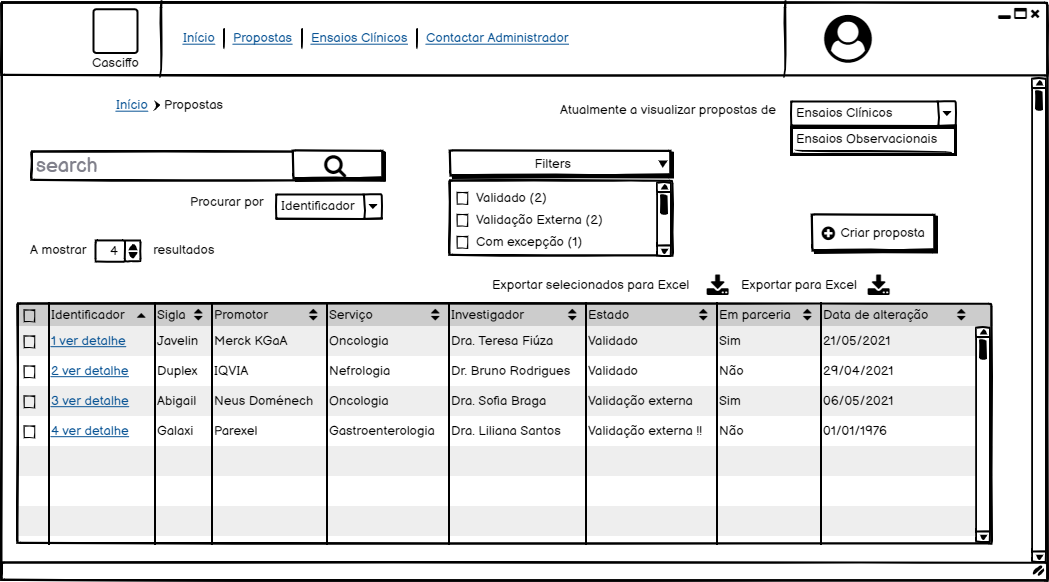
\includegraphics[scale=0.35]{images/proposals.png}
    \caption{Mock overview of clinical investigations proposals.}
    \label{fig:propostas}
\end{figure}

\begin{figure}[H]
    \centering
    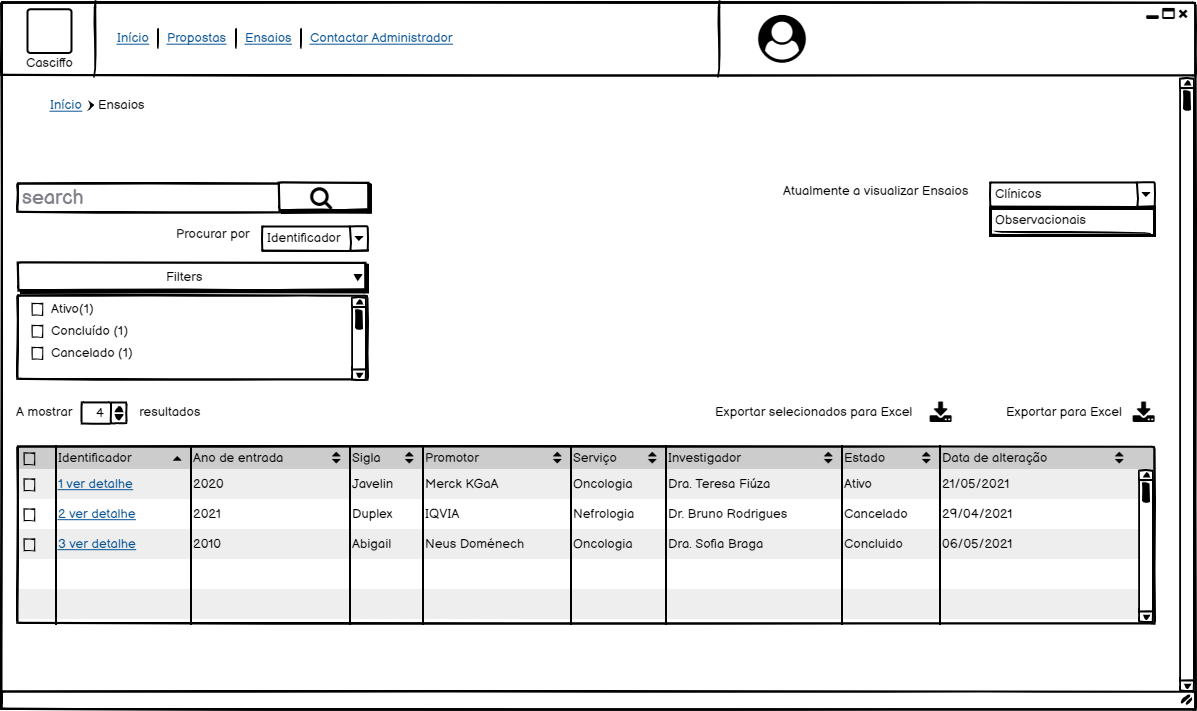
\includegraphics[scale=0.35]{images/ensaios.png}
    \caption{Mock overview of clinical trials.}
    \label{fig:ensaios}
\end{figure}


When a user clicks the link view details ("ver detalhe"), he will be redirected to a screen displaying the details of the target clinical investigation.

\subsection{Ability to edit and validate data (edit checks)}
\label{subsec:abilitiy-to-edit}
Within the CASCIFFO platform, the UIC and internal departments can view the details of a certain clinical investigation proposal and edit or validate according to their roles.
Users with `UIC` role will be able to create and edit their own Investigations, whereas the internal departments, with roles of `CA`, `Finance` and `Juridical` will only be able to validate the proposals.  
The creation of a proposal starts in the overview of proposals screen, from there a user can click on Create Proposal ("Criar proposta") and will be redirected to the screen illustrated in figure~\ref{fig:criar-proposta}. Here an investigator can choose what type of investigation this proposal corresponds to, either an observational or clinical trial. In the case a clinical trial is selected, more options will be shown since clinical trials have a corresponding financial component.
The data fields corresponding to the therapeutic area, the service and the pathology of an investigation are restricted to a set of possible inputs. In addition, the members of a medical team also belong to an already defined database, being validated at the time of creation of the medical team for the investigation.  
Certain fields cannot be changed once a proposal has been submitted, such as the promoter, the partnerships and the type of investigation can only be defined during the creation of a proposal.  


\begin{figure}[H]
    \centering
    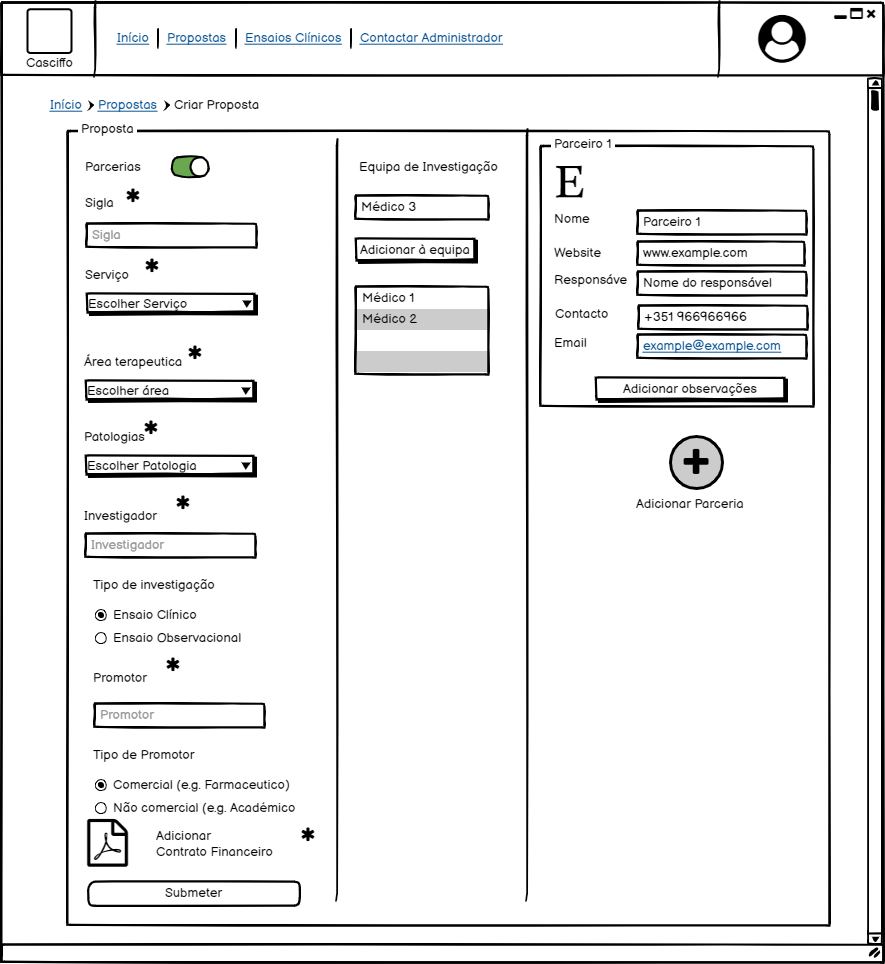
\includegraphics[scale=0.35]{images/criar-proposta.png}
    \caption{Mock creation of a clinical investigation proposal.}
    \label{fig:criar-proposta}
\end{figure}

\subsection{Access control based on different user profiles}
\label{subsec:access-control-based-user-profiles}
The access control within the CASCIFFO application is based on roles.
As described in section 1, there are defined roles for each type of user.  
A user with the role `UIC` can manage their own clinical investigation, being able to edit and have a hand in advancing the state. In addition, it also has an overview over all ongoing investigations, not being able to edit those that weren't created by said user. Once this user logs in, a dashboard showing overall statistics of the platform, \textit{i.e.} number of active clinical trials, number of submitted proposals, etc.
The role `Financial` is responsible for validating and updating the financial components of the investigations, hence when a user with this role logs in, an appropriate financial management screen will be displayed, whereas the `Juridical` component validates the juridical component.  
The role `CA` is responsible for giving the final decision in whether an investigation proposal can have the go-ahead to begin their clinical trials or observations.  
A user of role `CA` once logged in, will be shown a primary screen displaying the overview of clinical investigation proposals awaiting validation.
Finally, we have the `Superuser` role, which besides having the ability to execute every mentioned action, it can also create new types of services, therapeutic areas and pathologies.


\subsection{Access by computer, tablet or smartphone}
\label{subsec:access-by-mobile-device}
CASCIFFO is a web-application which can be accessed via any device or browser. CASCIFFO offers an extended functionality to browsers that support service workers, since it utilizes the Progressive Web Application (PWA) framework, allowing it to be installed and used as an application.
Among the features a PWA allows, the framework was chosen by its ability to let an application run in offline-mode and versatility in that it can be installed via the browser, and used in similarity to a standalone mobile app. 

\subsection{Ability to export information in numerical or graphical mode}
\label{subsec:ability-to-export-info}
CASCIFFO offers the ability to export information via excel, and visualize graphic data within the app.  
There is a feature, shown in figure~\ref{fig:proposta-export-excel} that allows a user to export data, \textit{e.g.} a selected number of clinical investigation proposals. This feature is present in the screens showing listed data, \textit{e.g.} list of clinical investigation proposals, and the details of each clinical investigation, proposal or trial.

\begin{figure}[H]
    \centering
    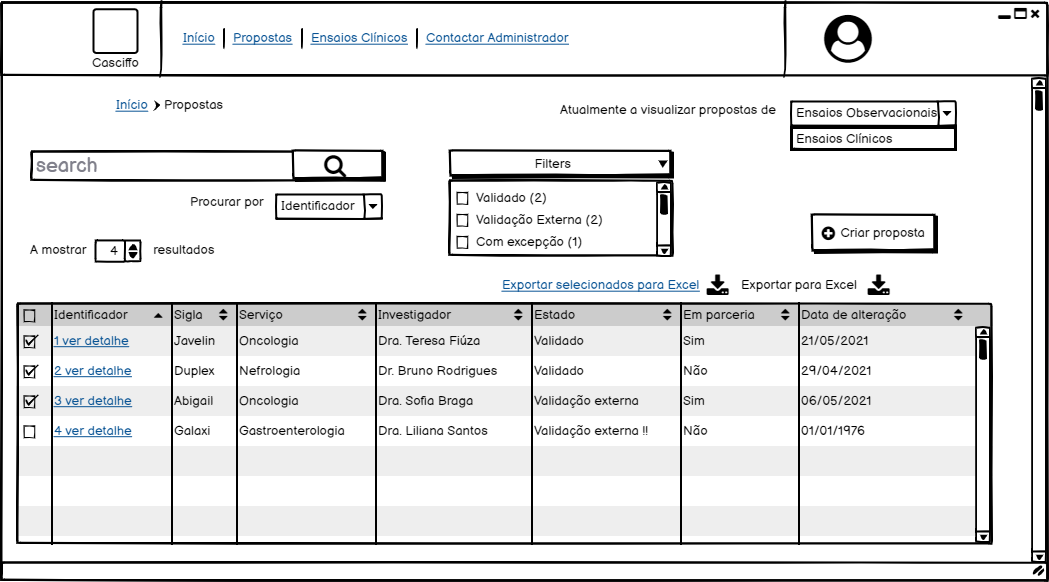
\includegraphics[scale=0.35]{images/propostas-exportar-para-excel.png}
    \caption{Mock screen selecting clinical proposals to export into excel.}
    \label{fig:proposta-export-excel}
\end{figure}

\subsection{Ability to customize the form of visualization}
\label{subsec:ability-to-customize-visualization}
The ability to customize the form of visualization will be available in the initial screen of the app, the Dashboard, where the user will be able to view different types of graphs showing statistics based on the states of clinical investigations.

\subsection{View detailed Characteristics and evolution of clinical Trials including the tested medicine or technique in question}
\label{subsec:clinical-investigation-details}
To view detailed information about a clinical investigation, one needs to first overview the clinical investigations and then click on the details of a desired clinical investigation. Considering this option, the user will be redirected to a screen detailing the study.  
The evolution of any clinical investigation consists of its proposal followed the trial activity once the proposal has been fully validated.
In figure~\ref{fig:proposta-detalhe}, the details of a clinical trial proposal can be viewed. The flow of state of a proposal is shown in the form of a bar in a straight forward manner. Each state corresponds to a division, box, in the bar and has three properties: the name of the State; the date it was completed in, if the state has otherwise not been completed, then a sequence of dashes will appear in its place; the deadline at which it should be completed and finally the entity responsible for advancing the state.  
It is possible to click in the box of a state to display information about the events that occurred during the time the proposal was in that state. 

\begin{figure}[H]
    \centering
    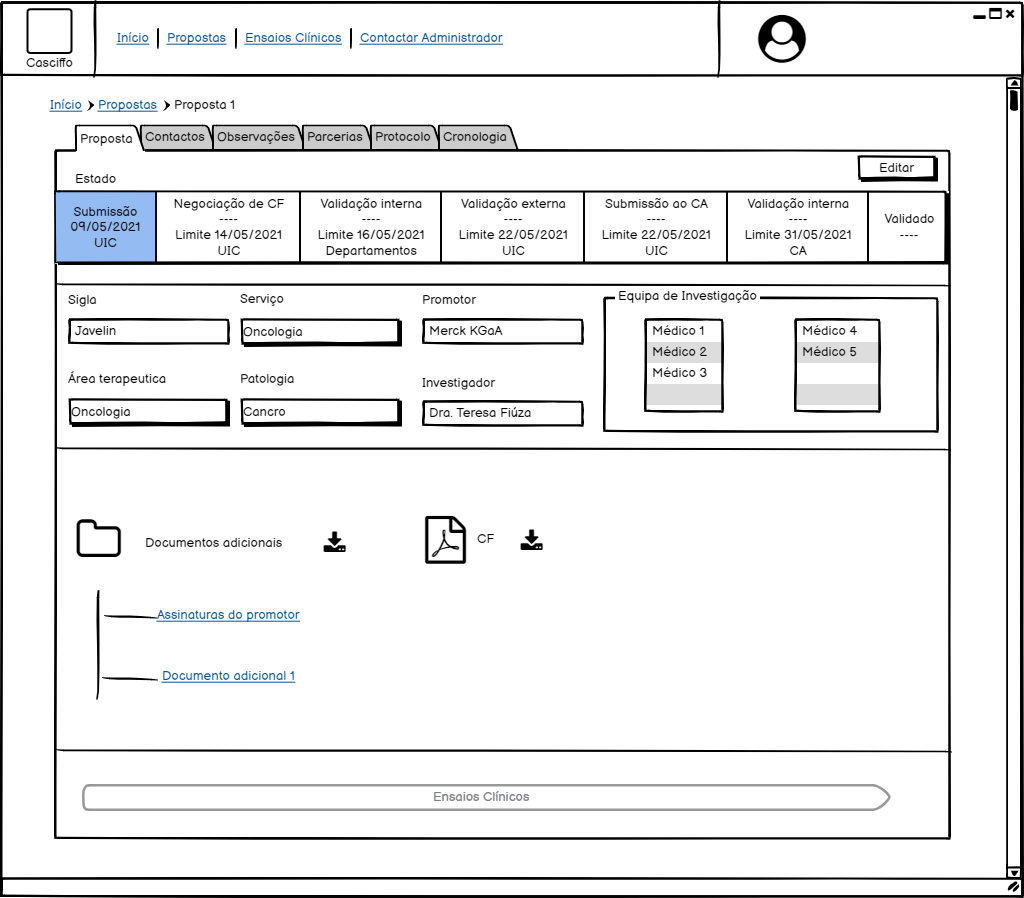
\includegraphics[scale=0.35]{images/proposta-detalhe.png}
    \caption{Mock overview of a clinical investigation proposal.}
    \label{fig:proposta-detalhe}
\end{figure}

A clinical trial proposal considers five components alongside its principal details displayed as tabs and listed below: 
\begin{itemize}
    \item the Contacts ("Contactos") tab which corresponds to comments related to external communications, viewed in figure~\ref{fig:proposta-contactos};
    \item the Observations ("Observações") tab which contains comments made in regard to the proposal, viewed in figure~\ref{fig:proposta-observações};
    \item the Partnerships ("Parcerias") tab, where one can find the partnerships involved in the study proposal, viewed in figure~\ref{fig:proposta-parcerias};
    \item the validation Protocol ("Protocolo") tab, where it can be viewed the current state of affairs of the process described in section~\ref{subsec:visualization-clinical-trials-as-process}, and in figure~\ref{fig:proposta-protocolo};
    \item the Chronology ("Cronologia") tab that displays the timeline of events, as in figure~\ref{fig:proposta-cronologia}. Events include deadlines introduced by the user and the transition of states. The user will have the ability to specify the scope of the timeline, selecting the time range and type of events to view. 
\end{itemize}

All tabs, except the one pertaining to the Protocol validation, will have present the current state of the proposal.

\begin{figure}[H]
    \centering
    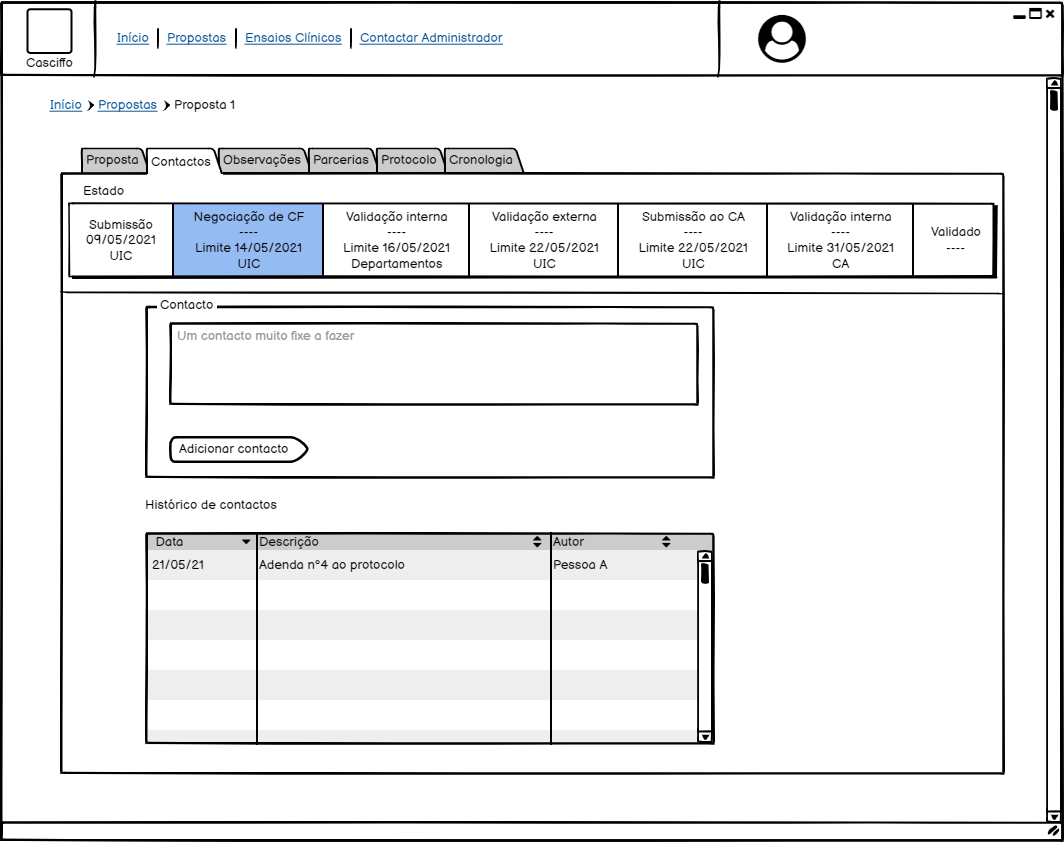
\includegraphics[scale=0.35]{images/proposta-contactos.png}
    \caption{Mock overview of the contacts tab.}
    \label{fig:proposta-contactos}
\end{figure}

\begin{figure}[H]
    \centering
    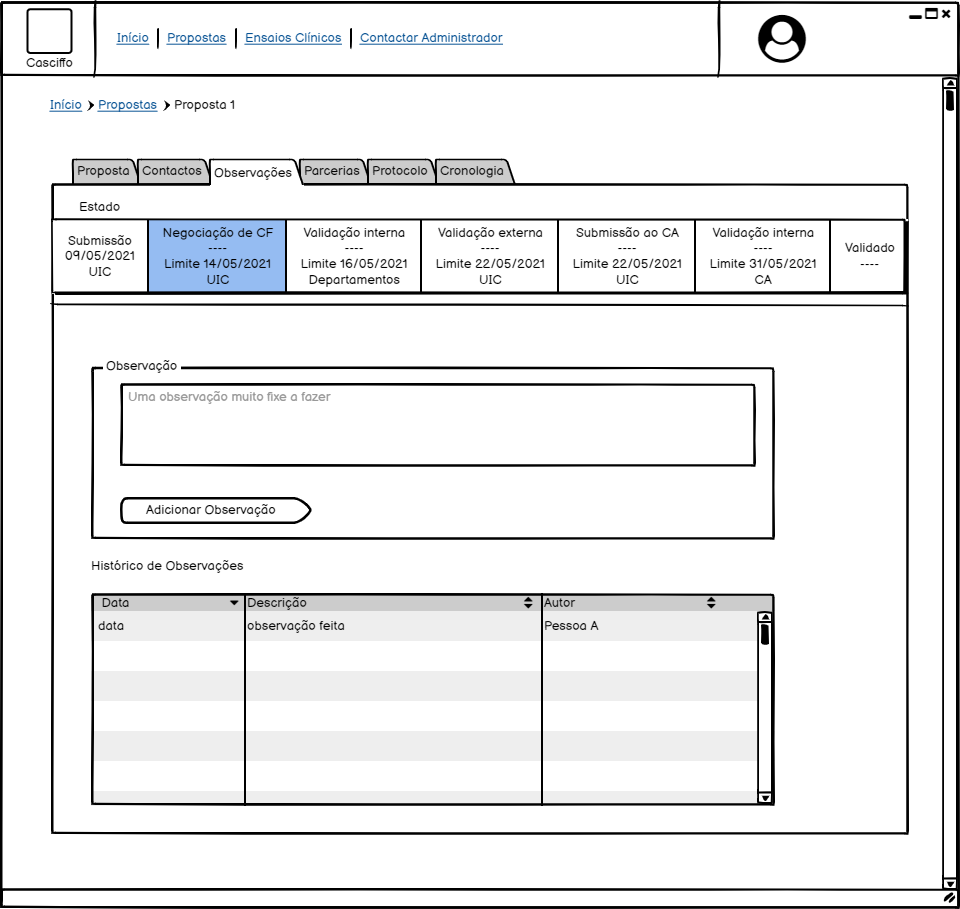
\includegraphics[scale=0.35]{images/proposta-observações.png}
    \caption{Mock overview of the observations tab.}
    \label{fig:proposta-observações}
\end{figure}

\begin{figure}[H]
    \centering
    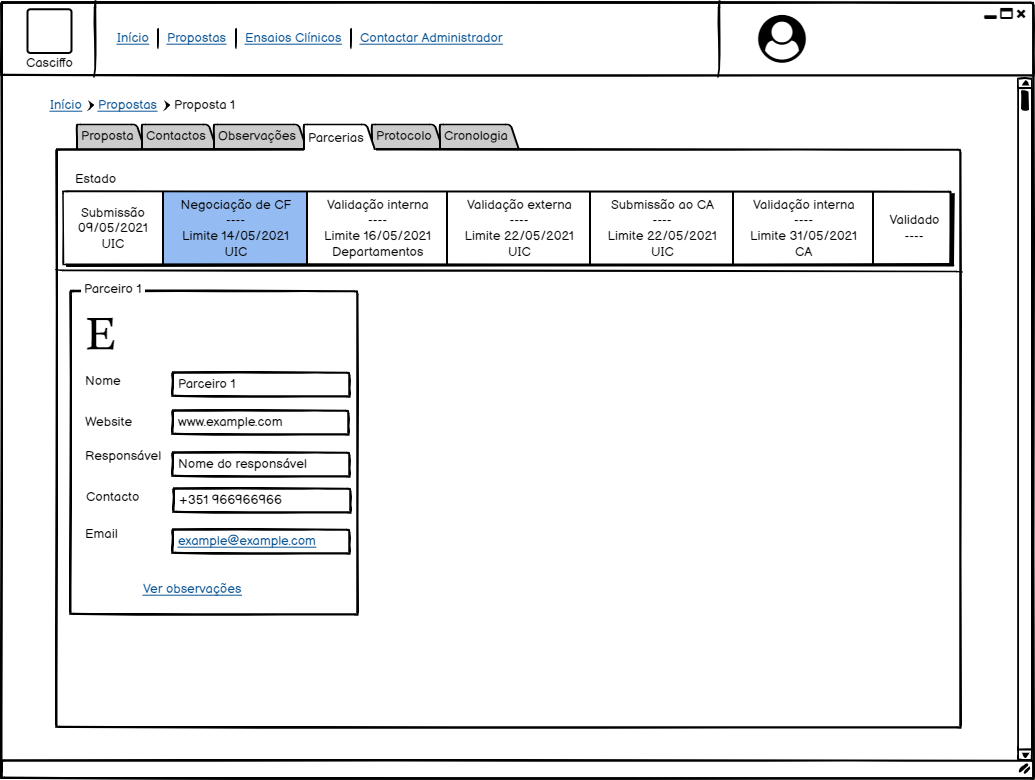
\includegraphics[scale=0.35]{images/proposta-parcerias.png}
    \caption{Mock overview of the partnerships tab.}
    \label{fig:proposta-parcerias}
\end{figure}

\begin{figure}[H]
    \centering
    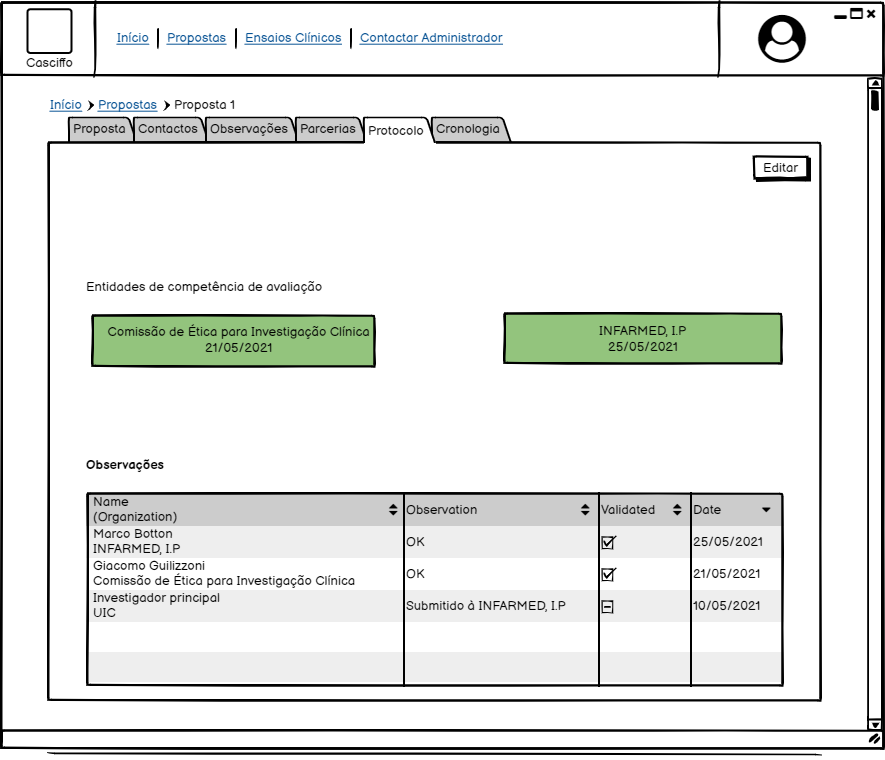
\includegraphics[scale=0.35]{images/proposta-protocolo.png}
    \caption{Mock overview of the protocol tab.}
    \label{fig:proposta-protocolo}
\end{figure}

\begin{figure}[H]
    \centering
    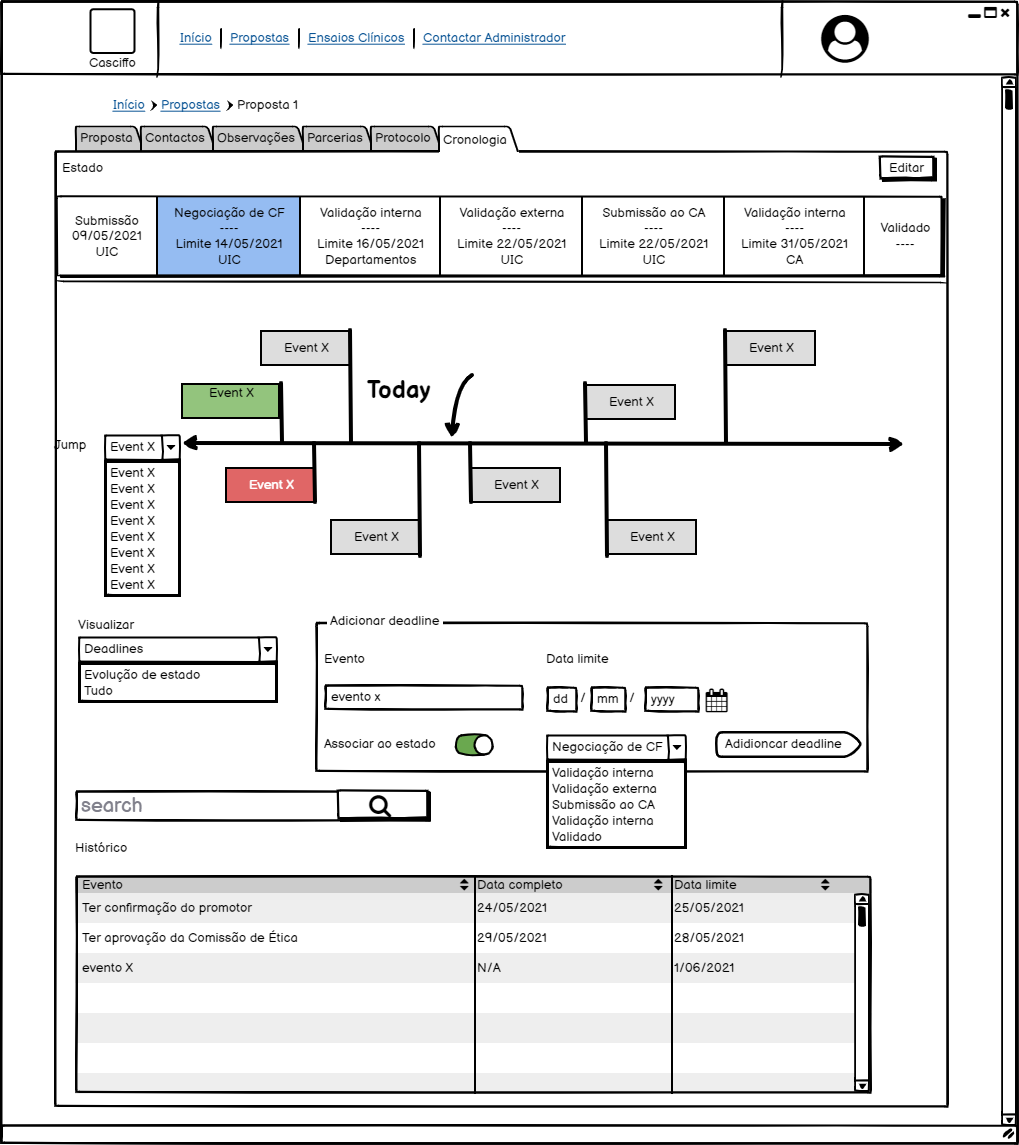
\includegraphics[scale=0.35]{images/proposta-cronologia.png}
    \caption{Mock overview of the chronology tab.}
    \label{fig:proposta-cronologia}
\end{figure}



Once the proposal has reached its successful terminal state, as in section~\ref{subsec:clinical-investigation-proposals} a clinical trial will be created. To access the newly created trial, the user can either click the button "Ensaio Clínico" from the proposal details screen, as in figure~\ref{fig:proposta-detalhe}, or from the overview of clinical trials click on the details of one.  
In the screen dedicated to the clinical trial and presented in figure~\ref{fig:enasio-detalhe}, there are five different tabs: 
\begin{itemize}
    \item the clinical trial tab ("Ensaio Clínico") that displays the characteristics of the study;
    \item the scientific activities tab ("Atividades científicas"), viewed in figure~\ref{fig:ensaio-atividades-cientificas}, which includes scientific work in the scope of the study, such as articles, thesis, reports, etc.;
    \item  the visits tab ("Visitas") where the investigator team can have an overview of the history and scheduled visits;
    \item the patients tab ("Pacientes") with the purpose of showing an overview of the participants included in the trial;
    \item the partnerships tab ("Parcerias"), similar to the proposal's version of partnerships tab, displays the partnerships involved in the study;
    \item the financial management ("Financiamento"), where one can view the flow of monetary gain from visits and the partition between the investigator team.
\end{itemize}

\begin{figure}[H]
    \centering
    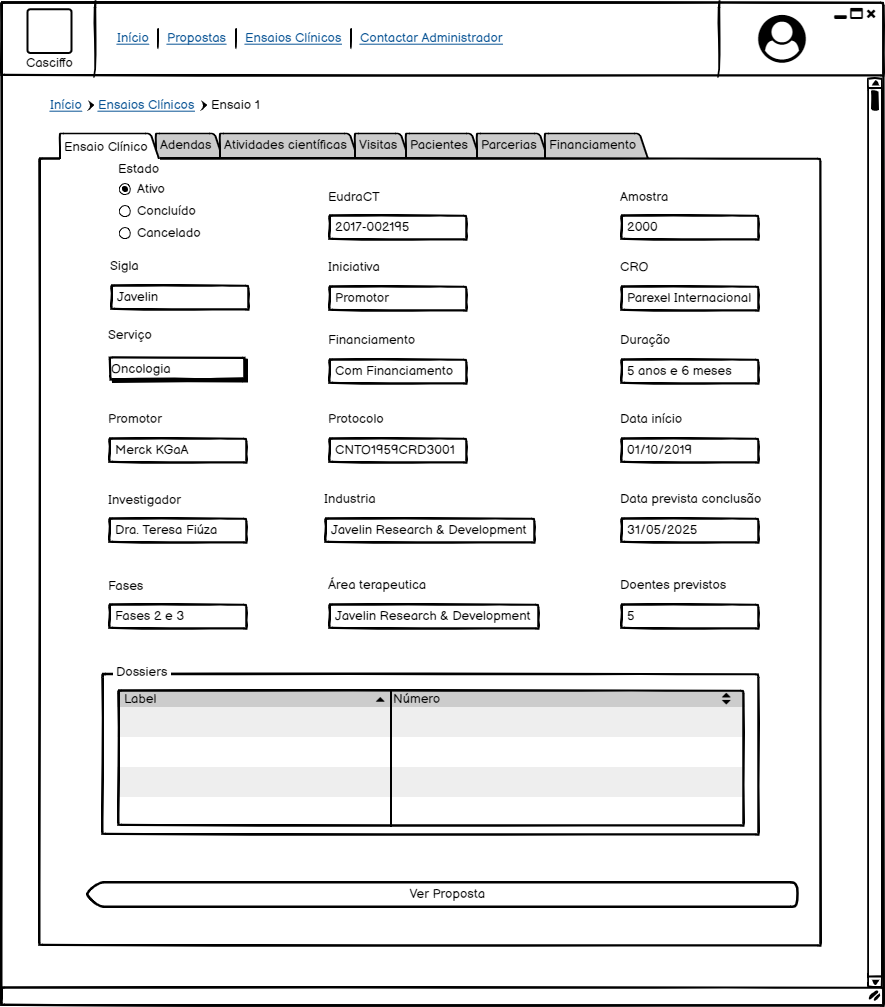
\includegraphics[scale=0.35]{images/ensaio-detalhe.png}
    \caption{Mock overview of the details of a clinical trial.}
    \label{fig:enasio-detalhe}
\end{figure}


\begin{figure}[H]
    \centering
    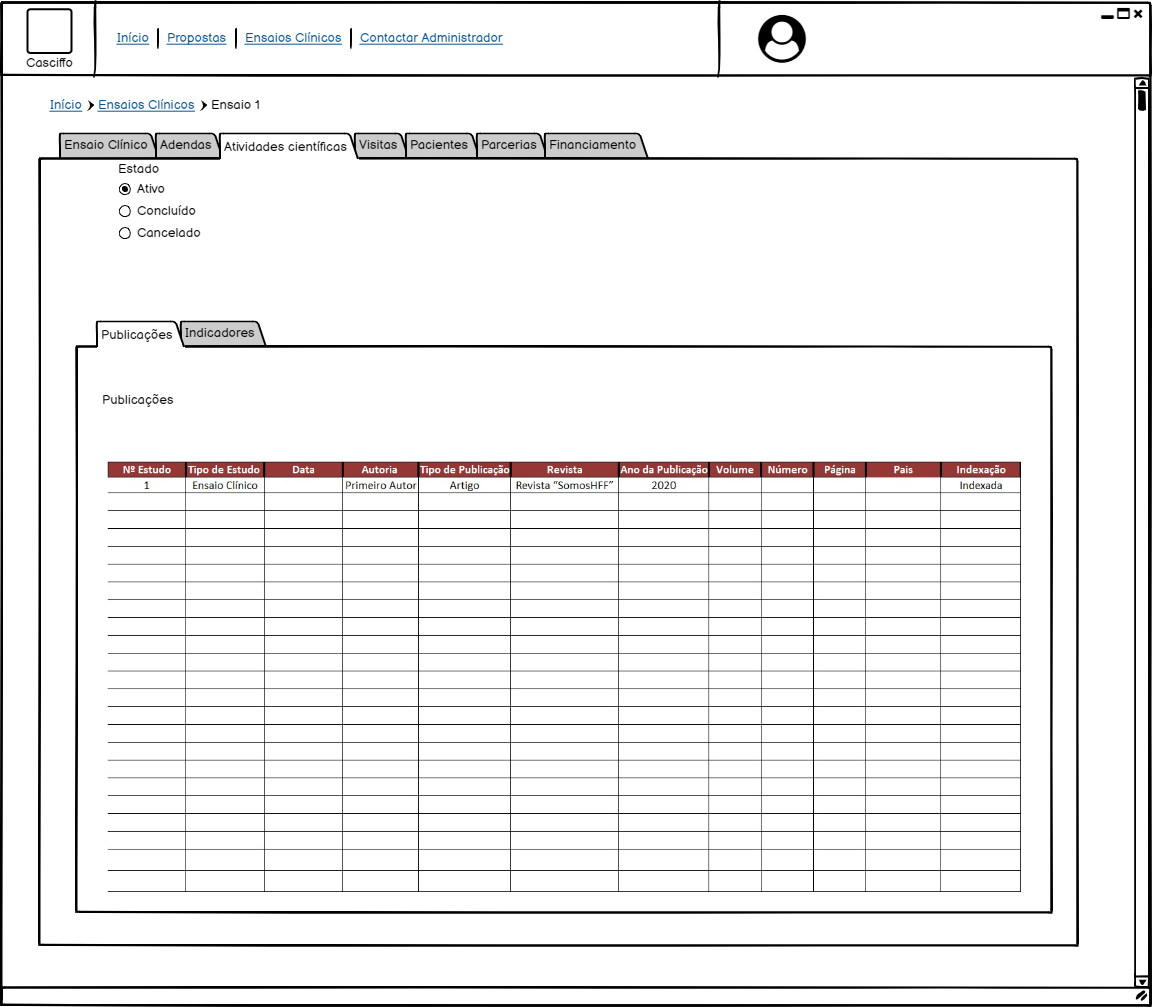
\includegraphics[scale=0.35]{images/ensaio-atividades-cientificas.png}
    \caption{Mock overview of scientific activities made within the scope of the investigation.}
    \label{fig:ensaio-atividades-cientificas}
\end{figure}


\subsection{Monitoring the set of patients included in clinical Trials and their characteristics}
\label{subsec:monitor-set-of-patients}
The details of the set of patients involved in a clinical trial will be displayed when viewing the details of said clinical trial, under the patients ("Pacientes") tab , illustrated in figure~\ref{fig:ensaio-participantes}. This tab displays the set of current participants undergoing the clinical trial and information such as the participant number, used to identify the participant throughout the study, the name of the participant, their age, the treatment branch they were assigned to within the scope of the study, their last and the closest upcoming visit.  
Included in this screen are the buttons Randomize ("Randomizar") and Add ("Adicionar").
The button "randomize" will randomly assign participants to treatment branches within the study, this one-time procedure is to be used once all the participants have been added to the clinical trial.
The button "add", will begin the procedure to add a patient. Upon clicking this button, the user will be shown a small box, as illustrated in figure~\ref{fig:ensaio-adicionar-paciente}, where he can input the name of the participant and then is also given the chance to immediately schedule several visits.

\begin{figure}[H]
    \centering
    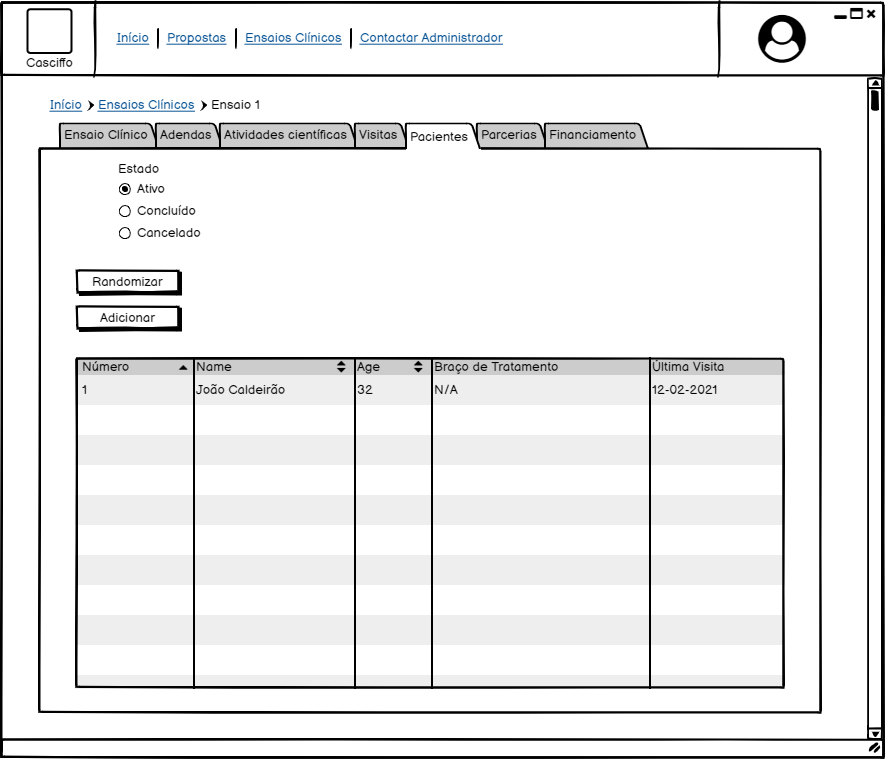
\includegraphics[scale=0.35]{images/ensaio-participantes.png}
    \caption{Mock overview of all participants included in the study.}
    \label{fig:ensaio-participantes}
\end{figure}

\begin{figure}[H]
    \centering
    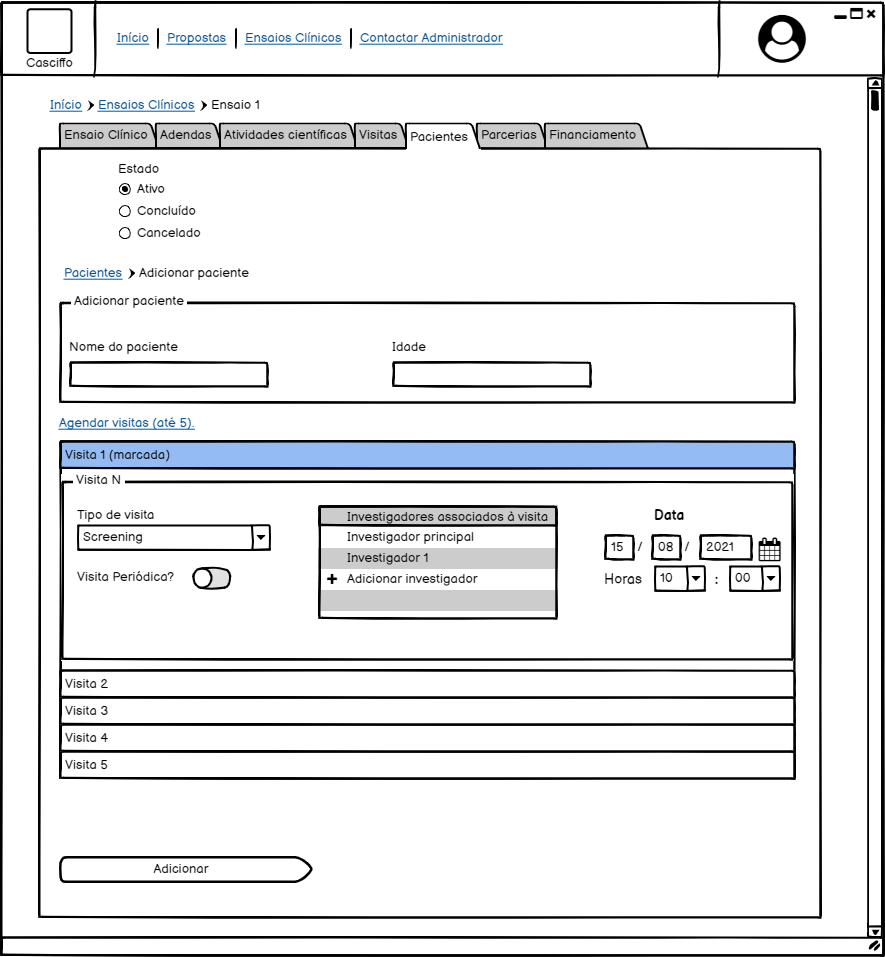
\includegraphics[scale=0.35]{images/ensaio-adicionar-paciente.png}
    \caption{Mock screen of adding a new patient as a participant in the study.}
    \label{fig:ensaio-adicionar-paciente}
\end{figure}

\subsection{Insertion of patient data in face-to-face or tele-consultation}

The insertion of patient data in the context of a visit is made by the investigator associated to the mentioned visit. In order to do this, the investigator has to navigate to the details of the visit, from the overview of clinical trials, to the details of the trial followed by the overview of visits and finally the details of the considered visit. Here the investigator can input observational data into the field "Observações" which will represent the observations made throughout the visit or tele-consultation. He is also asked to mark the attendance of the participant by clicking on a simple button "Marcar presença", as illustrated in figure~\ref{fig:ensaio-visita-detalhes}.

\begin{figure}[H]
    \centering
    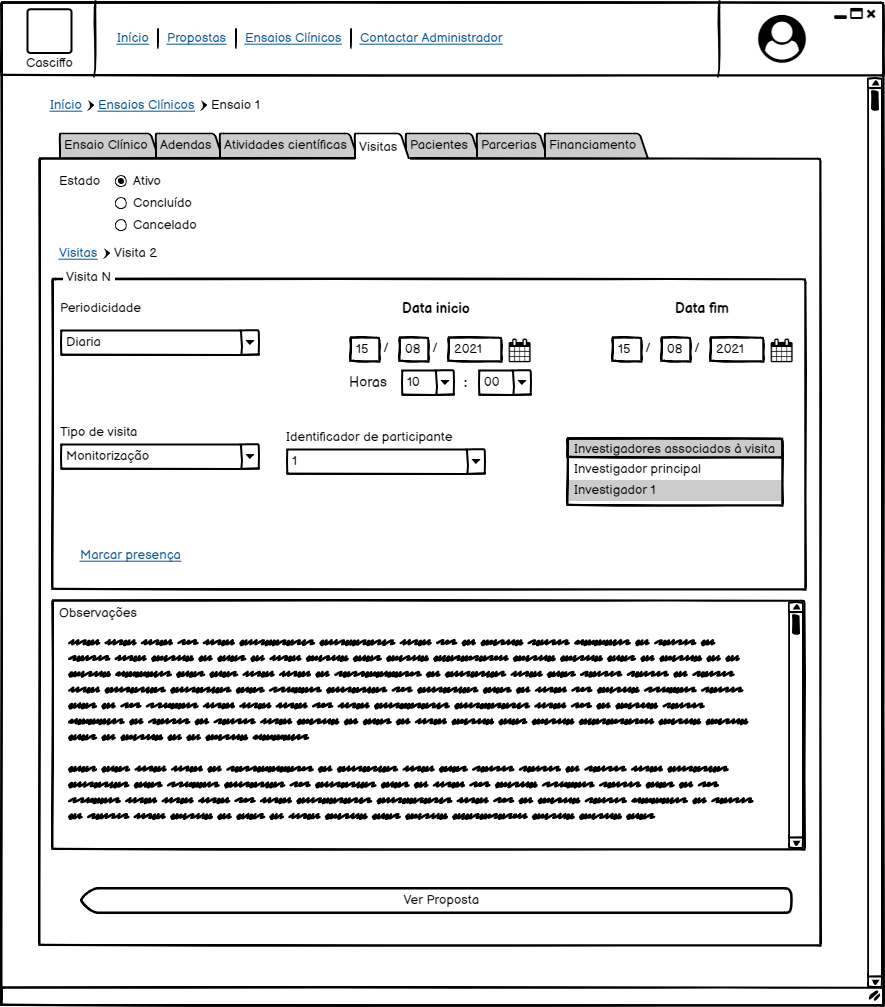
\includegraphics[scale=0.35]{images/ensaio-visita-detalhes.png}
    \caption{Mock overview of a visit's details.}
    \label{fig:ensaio-visita-detalhes}
\end{figure}
%TODO [ideia-colocar-eventos-mais-proximos-na-dashboard]


\subsection{Characteristics of the treatment associated with the clinical trial}
The characteristics of the treatment associated with clinical trials consists of three main factors, the service area it is within, the therapeutic field and the pathology the clinical trial aims to investigate/treat. These details can all be found in the detailed view of a clinical trial under the tab "Ensaio Clínico".  

\subsection{Monitoring of the patient’s behavior under trial and its attendance}
The monitoring of the patient's behavior and its attendance, can be tracked via the visits and in twofold. The first is to filter the visits, under the visits tab, to show only the visits related to the participant in question. The second is to view the details of this participant in particular, from the overview of total participants in the study, clicking on the details of the participant and then checking the tab "Attendance", as in figure~\ref{fig:ensaio-paciente-detalhes}. 

\begin{figure}[H]
    \centering
    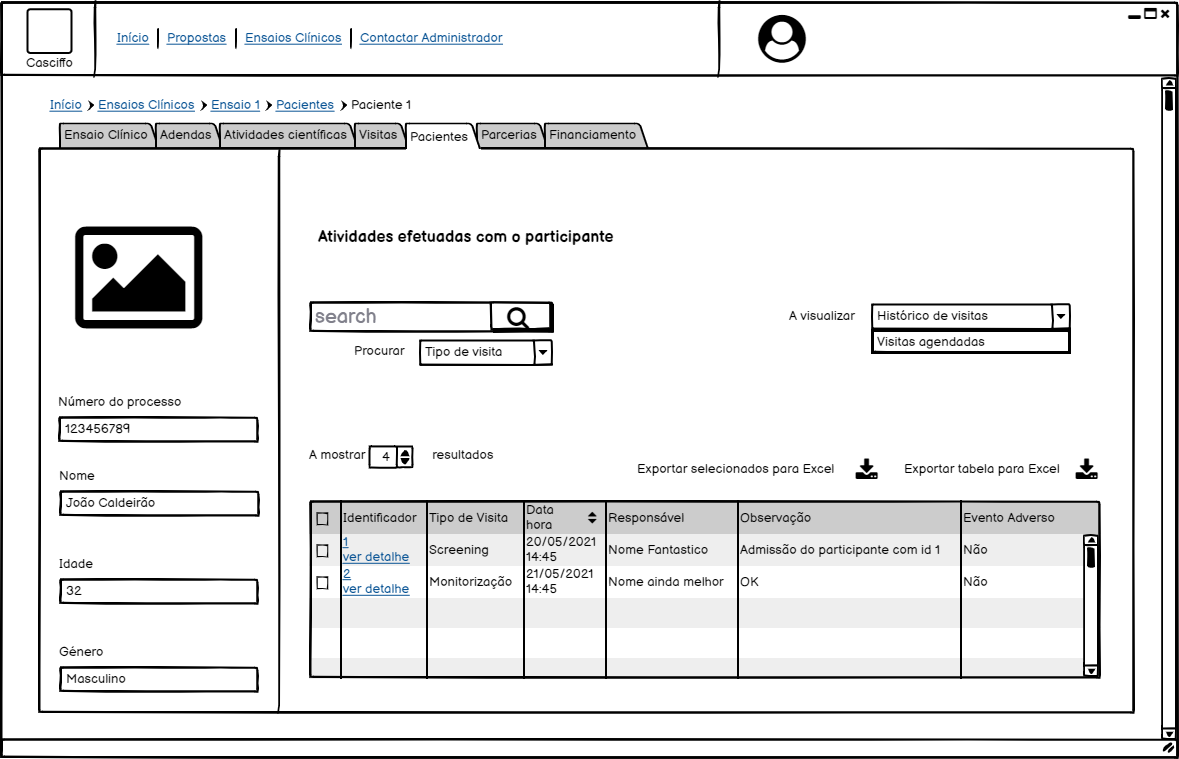
\includegraphics[scale=0.35]{images/ensaio-paciente-detalhes.png}
    \caption{Mock overview of patient details.}
    \label{fig:ensaio-paciente-detalhes}
\end{figure}

\subsection{Monitoring of physical and financial assets} 
In regard to the monitoring of physical assets, these can be viewed under the tab "Ensaio Clínico" while in the detail page of the clinical trial in question. The assets to be monitored are documentation archives, consisting of three fields: the Volume, a Label and the total Number.
CASCIFFO also offers another type of monitoring, the monetary flow. As described in section~\ref{subsec:clinical-trials}, each clinical trial has a financial management section that discriminates the earnings made by visit and the partitions of each team member involved in the study.  
Under the tab "Financiamento", the general monetary information, such as, total balance ("saldo"), amount per participant, etc., is displayed on a top section of the page. Below this section it can be observed another two tabs, differentiating the income made from the investigation team and the clinical trial itself. The first tab "EC", shown in figure~\ref{fig:ensaio-finance-ec}, shows the income made according to the visits done, whereas the second tab "Equipa", illustrated in figure~\ref{fig:ensaio-finance-team}, shows the income by team member.

\begin{figure}[H]
    \centering
    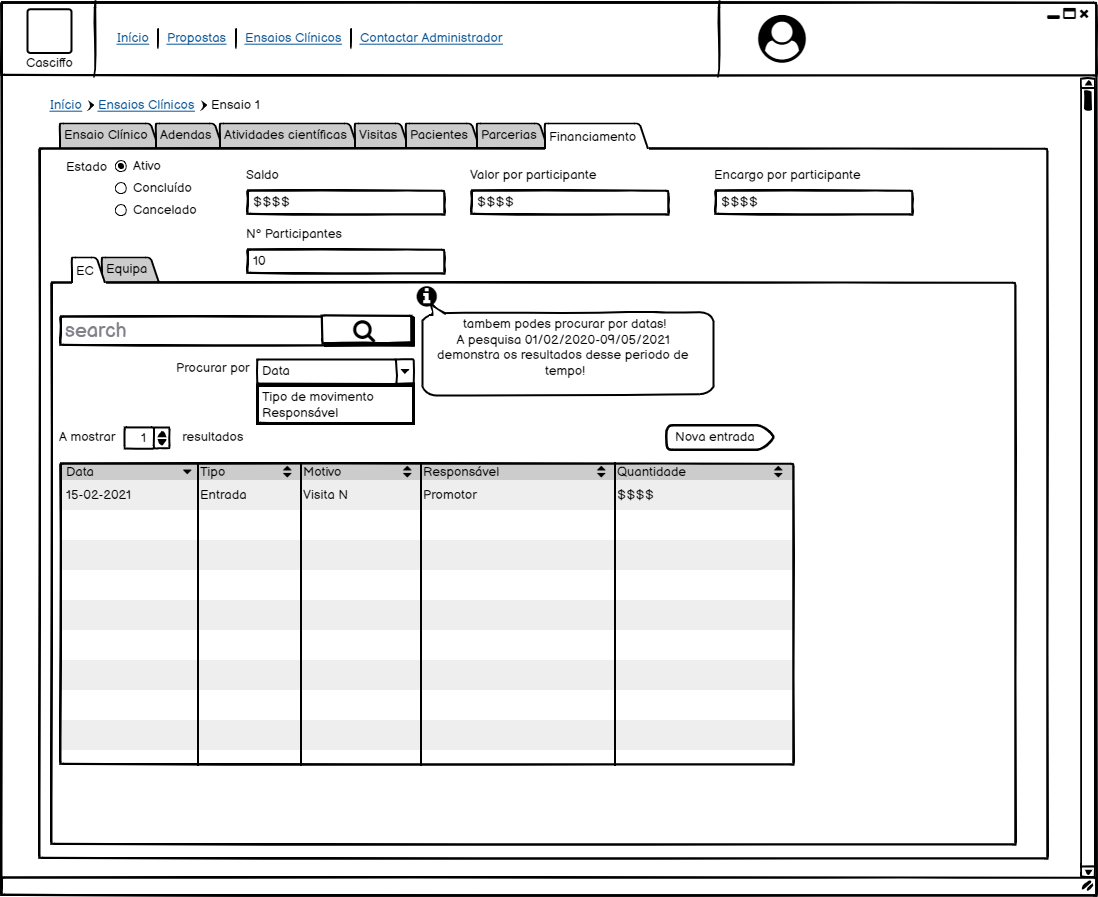
\includegraphics[scale=0.35]{images/ensaio-finance-ec.png}
    \caption{Mock detailed view of the income flow made in the investigation.}
    \label{fig:ensaio-finance-ec}
\end{figure}

\begin{figure}[H]
    \centering
    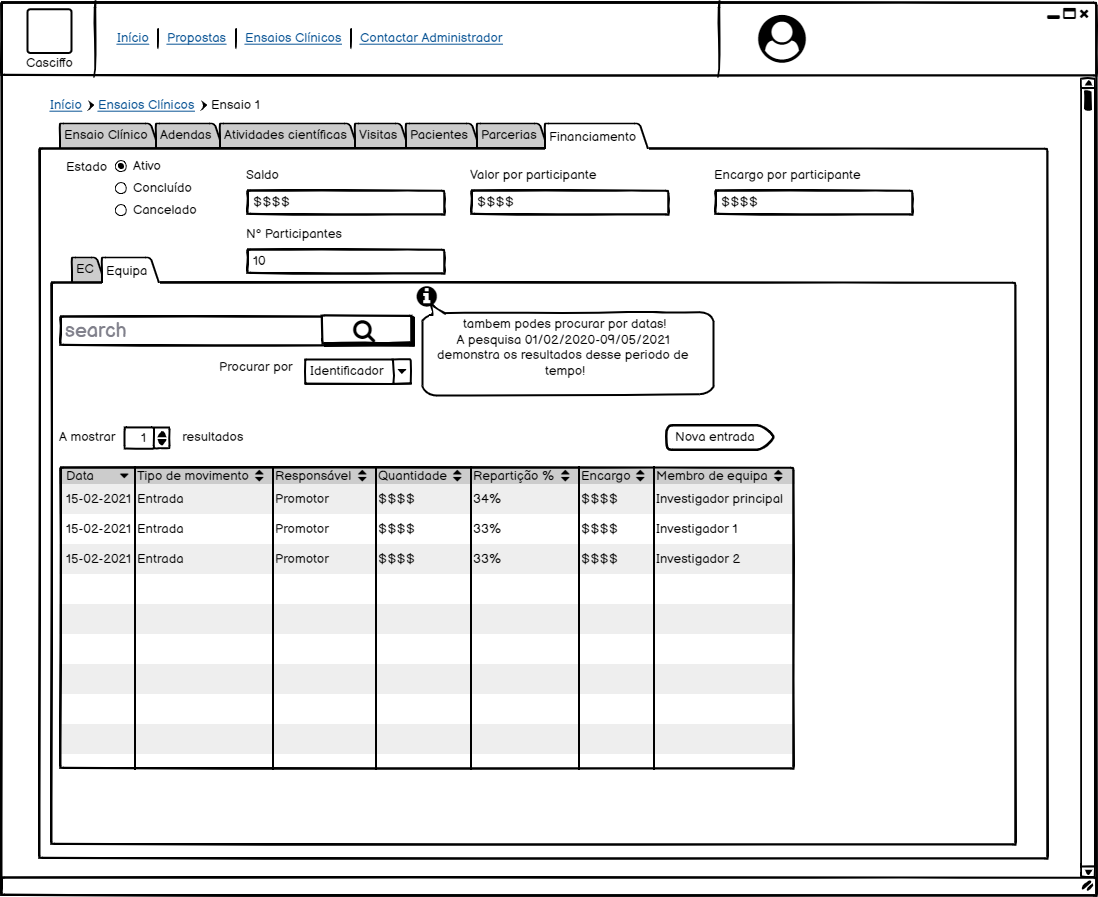
\includegraphics[scale=0.35]{images/ensaio-finance-team.png}
    \caption{Mock detailed view of income flow divided by the investigator team.}
    \label{fig:ensaio-finance-team}
\end{figure}

\subsection{Monitoring of visits \& recording of adverse events} 
The monitoring of visits during a clinical trial can be tracked and viewed under the tab "Visitas", in the detailed screen of a clinical trial.
In this setting, any investigator (associated to the clinical trial) is able to view and track the past and scheduled visits made by the team. However, only the investigators associated to a visit are able to manipulate them. When creating a visit, that visit will automatically be associated to its creator, giving also the option to associate other investigators to the same visit, allowing them to freely edit the visit details. Along with this option, the investigator is required to fill in the fields depicted in figure~\ref{fig:ensaio-visitas}. These fields are as follows: the periodicity ("Períodicidade") that can be turned ON in case the visit is a reoccurring one with the ability to schedule at a custom interval in days; the type of visit ("Tipo de visita"), that has three possible inputs, Screening, indicating the first visit, Monitoring ("Monitorização") indicating a motoring visit and finally a Closeout visit, which indicates the final visit done to a participant. In case the visit is periodic, the field of `end date` ("Data fim") becomes mandatory to fill.  

\begin{figure}[H]
    \centering
    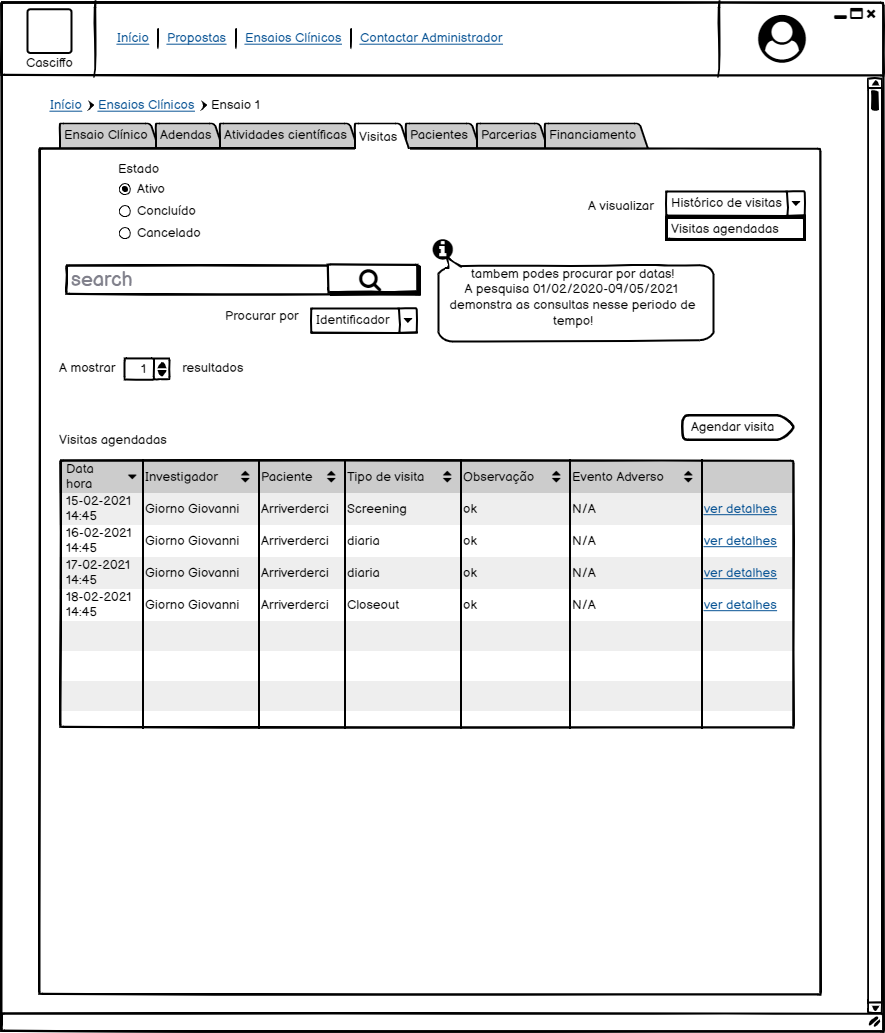
\includegraphics[scale=0.35]{images/ensaio-visitas.png}
    \caption{Mock overview of visits scheduled in the clinical trial.}
    \label{fig:ensaio-visitas}
\end{figure}

When a visit occurs, the associated investigators will have access to the observations ("Observações") field and adverse event ("Evento adverso") warning. In addition to this, the field "Marcar presença" is now available to mark attendance.